\documentclass[12pt]{article}
\usepackage[none]{hyphenat}
\usepackage{amsmath}
\usepackage{float}
\usepackage{graphicx}
\usepackage{atbegshi}
\AtBeginDocument{\AtBeginShipoutNext{\AtBeginShipoutDiscard}}
\newcommand{\solution}{\noindent \textbf{Solution: }}
\providecommand{\brak}[1]{\ensuremath{\left(#1\right)}}
\newcommand{\myvec}[1]{\ensuremath{\begin{pmatrix}#1\end{pmatrix}}}
\let\vec\mathbf
\begin{document}
\graphicspath{{./Documents}{./figs}}
\begin{center}
  \title{\textbf{Linear Forms}}
  \date{\vspace{-5ex}}
  \maketitle
\end{center}
\setcounter{page}{1}
\section*{11$ ^{th} $ Maths - Chapter 10}
The following problem is question 13 from exercise 10.3:
\begin{enumerate}
  \item Find the equation of the right bisector of the
 line segment joining the points (3, 4) and (–1, 2).
\end{enumerate}
\solution \\
Given that \\
\begin{align}
(x_1 , y_1) = (3 , 4)
\label{p:1} \\
(x_2 , y_2) = (-1 , 2) 
\label{p:2}
\end{align}
The midpoint (x , y) is given by. 
\begin{align}
	m (x , y) &= \left( \frac{x1 + x2}{2} , \frac{y1 + y2}{2}\right)\\
	      &= \left( \frac{3 - 1}{2} , \frac{4 + 2}{2} \right )\\
	      &=( 1 , 3 ) \label{p:5}
\end{align}
The direction vector of a line containing two points \eqref{p:1} and
\eqref{p:2} is given by.
\begin{align}
	\vec{V} &=
	    \myvec{x2 & -x1 \\ \\ y2 & -y1} 
    \end{align}
    \begin{align}
	    &=
		 \myvec{ -1 & -3 \\ \\ 2 & 4}
    \end{align}
    \begin{align}
        =
		   \myvec{-4 \\ \\ -2}
    \end{align}
    The direction vector of right bisector is given by.
    \begin{align}
	    \vec{V_{perpendicular}} &=
		  \myvec{2 \\ \\ -4}
    \end{align}
    The position vector $\vec{P}$ at \eqref{p:5} of line is given by.
	    \begin{align}
			    \myvec{x & -1 \\ \\ y & -3}
	    \end{align}
    The equation of line in vector form is given by.\\
    \begin{align}
         \vec{V} . \vec{P} = \vec{V_{perpendicular}} . M
    \end{align}
    \begin{align}
	    \myvec{-4 \\ \\ -2} 
	    \myvec{x & -1 \\ \\ y & -3}
    =
	    \myvec{ 2 \\ \\ -4}
	    \myvec{1 \\ \\ 3}
    \end{align}
    By simplifying this, we get
    \begin{align}
        2x + y = 5
    \end{align}
    Therefore, the above equation can be written as
    \begin{align}
	    \myvec{2 & 1}\vec{x} = 5
    \end{align}

    \begin{figure}[H]
  \centering
  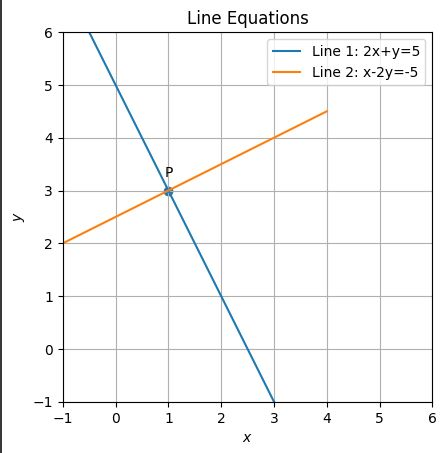
\includegraphics[width=\columnwidth]{figs/graph.jpg}
  \caption{Graph}
  \label{fig:pic}
\end{figure}
\end{document}
